\section{Results - Titan \label{sec:results_Titan}}

The following results are split into three main sections. We firstly present specific solutions to the LTEs for a global surface ocean on Titan using Rayleigh friction. We then compare dissipation between the analytical and numerical solutions in section \ref{subsubsec:linTitan}. Section \ref{subsec:botTitan} then presents purely numerical results for dissipation using only bottom friction. These results are then repeated for Enceladus in section \ref{sec:results_Enceladus}.

\subsection{Rayleigh Friction}

\subsubsection{LTE Solutions}

Figure \ref{fig:LTE_solns} illustrates numerical solutions to the LTE, at periapse, for different components of the tidal potential on Titan. Surface displacement, $\eta$, is illustrated on the left, whereas velocity, $\bm{u}$, is on the right. The colour scale in the velocity figures represents the velocity's magnitude, $\left| \bm{u} \right|$. Arrows indicate the direction of flow. The tidal forcing applied is, from a) to c), the eccentricity tide, obliquity tide, and full tide, respectively. All plots are for the ``canonical'' $400 \, \si{\metre}$ ocean used by \citet{sagan1982tide} for best comparison with \citet{sears1994tidal,sears1995tidal,sohl1995tidal}.

Surface displacement in Figure \ref{fig:LTE_a} shows a classic tidal bulge, centered on the Saturnian ($\phi = 0^{\circ}$) and sub-Saturian ($\phi = 180^{\circ}$) points. Maximum displacement is over $8$ metres. Away from the tidal bulge, displacement drops below the equilibrium level to less than $4$ metres. The corresponding flow shows convergence and divergence at the longitudinal positions of steepest gradient in the displacement field. Fastest flow occurs at the maxima and minima of the displacement.

The obliquity tide shows markedly different displacement and flow patterns than the eccentricity tide (Figure \ref{fig:LTE_b}). Displacement is now anti-symmetric about the equator. Notably, the longitudinal positions of maxima and minima are offset from the Saturnian and sub-Saturnian points. The tide raised by the obliquity tidal potential is also an order of magnitude less than the eccentricity tide. Flow is mainly poleward, converging south of the equator on the Saturn-facing hemisphere, and north of the equator on the opposite hemisphere.

The final plot in figure \ref{fig:LTE_solns} is the solution under the full tidal potential. In many ways, it is similar to the eccentricity tide. Yet, the addition of the obliquity tide adds significant equatorial asymmetry to the solutions. This asymmetry is particularly noticeable in the velocity plot on the right hand side of Figure \ref{fig:LTE_c}, where the areas of fastest flow are skewed north and south of the equator, unlike in Figure \ref{fig:LTE_a}. This is also evident in the displacement field, where the highest tide is offset from the equator.

These simulations were run from undisturbed initial conditions: \hbox{$\eta = 0 \, \si{\metre}$} and \hbox{$\bm{u} = (0,0) \, \si{\metre\per\second}$}. Consequently, there was some start-up time required for the model to converge into its orbitally-averaged equilibrium, as noted by \citet{sears1995tidal}. Figure \ref{fig:conv_a} illustrates this type of behaviour.

\begin{figure*}[!t]
\centering
\begin{subfigure}{0.9\linewidth}
\centering
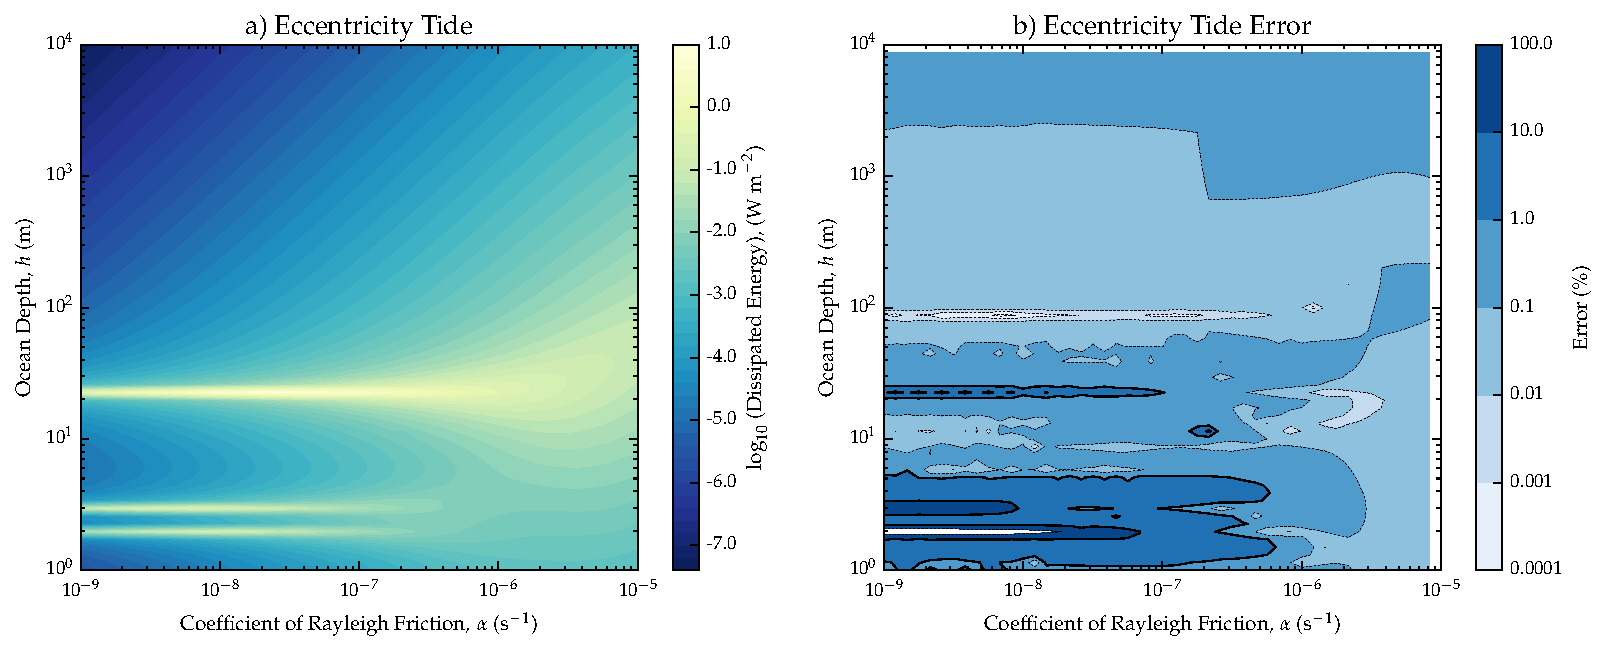
\includegraphics[width=\linewidth]{Figures/Eccentricity_error}
\subcaption{\label{fig:lincEccTitan}}
\end{subfigure}\\\vspace*{-0.5cm}
\begin{subfigure}{0.9\linewidth}
\centering
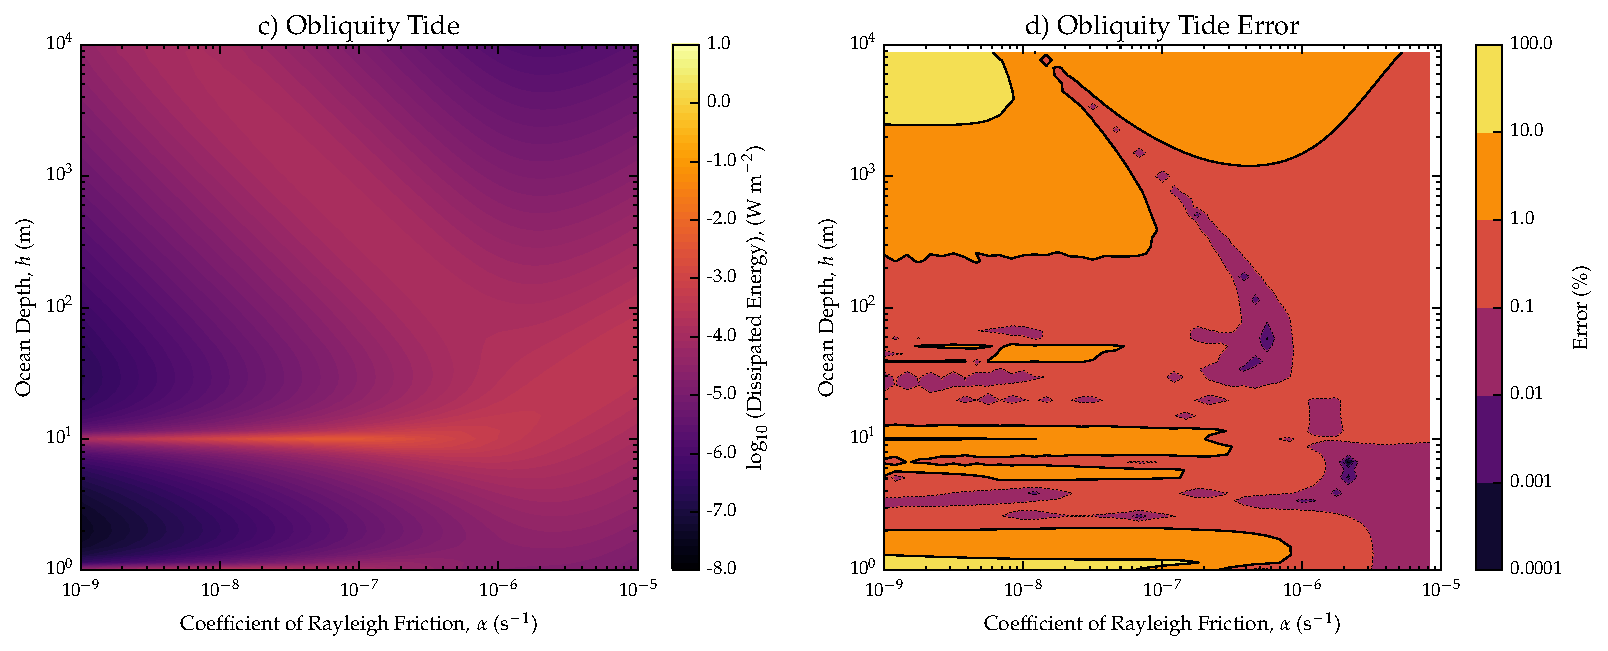
\includegraphics[width=\linewidth]{Figures/Obliquity_error}
\subcaption{\label{fig:linObliqTitan}}
\end{subfigure}
\vspace*{-0.8cm}
\caption{Numerical global surface ocean dissipation solution for Titan under the eccentricity and obliquity tides. The logarithm of dissipated energy is shown as function of ocean depth, $h$, and Rayleigh friction coefficient, $\alpha$, on the left hand side of the figure. The numerical error for each tidal component is then shown in the right hand plots. All simulations were performed with $\ang{2}$ grid spacing. \label{fig:linTitan}}
\end{figure*}

\subsubsection{Tidal Dissipation \label{subsubsec:linTitan}}

Orbitally averaged dissipated energy was derived for over 3000 simulations using equations \ref{eq:E_alpha} and \ref{eq:E_alpha_orbit} over a range of $h$ and $\alpha$ values for each main tidal component as shown on the left hand side of Figure \ref{fig:linTitan}. The eccentricity tide (Figure \ref{fig:lincEccTitan}) shows three resonant dissipative ocean thicknesses, $h \sim$ \SIlist{2;3;22}{\metre}. These deepest of these resonances has a maximum dissipated surface heat flux of $\sim 10\, \si{\watt\per\square\metre}$, which occurs between $\alpha =$ \SIlist{e-8;e-7}{\per\second}. Notably, the maximum dissipated energy does not occur for the most friction dominated oceans where $\alpha \sim \num{e-5} \, \si{\per\second}$.

Figure \ref{fig:lincEccTitan} illustrates the orbitally averaged surface heat flux for the obliquity tides on Titan. Two resonant ocean thicknesses are found for this tidal component, $h \sim$ \SIlist{1;10}{\metre}. The latter resonance is the most dissipative with an average surface heat flux of $\sim \num{4e-3}\, \si{\watt\per\square\metre}$.


\subsection{Bottom Friction \label{subsec:botTitan}}

\section{Results - Enceladus \label{sec:results_Enceladus}}

\subsection{Scaling Laws \label{subsec:scaling}}